\documentclass[a4paper, 12pt]{article}
\usepackage[french]{babel}
\usepackage[utf8]{inputenc}
\usepackage[T1]{fontenc}
\usepackage{lmodern}
\usepackage{graphicx}
\usepackage{listings}
\usepackage{color}

\lstset{language=C,rangeprefix=//---------------,rangesuffix=----------------,includerangemarker=false,columns=spaceflexible,extendedchars=true,showspaces=false,showstringspaces=false,inputencoding=ansinew,tabsize=4,frame=shadowbox,morecomment=[is]{\#ifdef}{\#endif},morecomment=[is]{/*}{*/}}

\title{Lecture et rédaction scientifiques: \\Skip-lists }
\author{Steve Zaretti}

\begin{document}
	
	\maketitle
	\newpage
	\tableofcontents
	\newpage
	
	\section{Introduction}
	\subsection{Liste chainée}
	Une liste chainée est une structure de données de taille arbitraire. Le principe est que chacun des éléments de cette liste contient une référence vers l'élément suivant. Cette pratique facilite l'insertion et la suppression des éléments, au détriment de la rapidité et de la recherche.
	
	\subsubsection*{Les alternatives}
	Il existe de nombreuses alternatives aux listes chainées pour trouver un élément plus rapidement: les tables de hashages, les arbres binaires, etc. Mais certaines séquences d'insertions peuvent être catastrophiques. Par exemple, insérer des éléments croissants dans un arbre binaire provoque un rééquilibrage de l'arbre. En revanche, si les éléments sont insérés de façon aléatoire, l'équilibrage devient plus rare.

	Grâce aux probabilités, les \og skip-list \fg{} bénéficient d'un atout majeur: aucune séquence ne peut provoquer systématiquement le pire scénario. Mieux encore, les skip-lists utilisent des algorithmes plus simples et rapides que ses concurrents. Les skip-lists sont aussi très légère et peuvent être configurée pour n'utiliser que $1\frac{1}{3}$ pointeurs par élément.
	
	\subsection{Skip-List}
	 Une skip-list bénéficie des avantages de la liste chainée, sans ses inconvénients. Cette structure de données utilise les chaines de façon parallèle. Une fonction basée sur des probabilités permet de déterminer si une nouvelle chaine doit être utilisée ou non. Cette couche supérieure est un moyen plus rapide d'accéder à cet élément.
	\begin{center}
		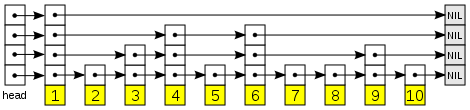
\includegraphics[width=\textwidth]{img/SkipList}
	\end{center}
	
	\subsubsection*{Définition}
	\begin{itemize}
		\item La hauteur maximale d'une skip-list est définie lors de sa création. Bien qu'il n'y ait pas de taille maximale d'une skip-list, il est conseillé d'utiliser $log_2(n)$ où $n$ est le nombre d'éléments théoriques présents dans la liste. 
		\item Le niveau le plus bas de la liste mène au nœud suivant. 
		\item Les nœuds supérieurs pointent vers un nœud plus avancé dans la liste.  Une couche supérieure est une voie rapide vers la couche inférieure. Ainsi, la couche la plus haute contient les sauts les plus grands.
		\item Le parcours d'une skip-list se fait de haut en bas, et de droite à gauche. Si la clé de l'élément suivant sur une couche est plus grande que celle qu'on recherche, celle-ci continue sur une voie inférieure.
		\item L'insertion dans la liste utilise une fonction de probabilité afin de définir sa hauteur maximale.
	\end{itemize}
	
	\section{Les algorithmes}
	\lstinputlisting[linerange=BEGINSKStruct-ENDSKStruct]{SkipList/SkipList.h}
	\subsection{La recherche}
	\lstinputlisting[linerange=BEGINSKSearch-ENDSKSearch]{SkipList/SkipList.c}
	\subsection{La hauteur}
	\lstinputlisting[linerange=BEGINSKRandom-ENDSKRandom]{SkipList/SkipList.c}
	\subsection{L'insertion}
	\lstinputlisting[linerange=BEGINSKInsert-ENDSKInsert]{SkipList/SkipList.c}
	\subsection{La suppression}
	\lstinputlisting[linerange=BEGINSKDelete-ENDSKDelete]{SkipList/SkipList.c}
	
	\section{Analyse des performances}
	\section{Comparaison avec d'autres structures de données}
	
	@online{1,
		author = {Patrice Roy},
		title = {Skip Lists},
		date = {27/02/2015},
		url = {http://h-deb.clg.qc.ca/Sujets/Structures-donnees/SkipLists.html},
	}
	@online{2,
		author = {Sylvie Hamel},
		title = {Dictionnaires ordonnés et “Skip List”},
		date = {25/02/2016},
		url = {http://www.iro.umontreal.ca/~hamelsyl/SkipList.pdf},
	}
	
\end{document} 